%%%%%%%%%%%%%%%%%%%%%%%%%%%%%%%%%%%%%%%%%%%%%%%%%%%%%%%%%%%%%%%%%%%%%%%%%%
%%%%%%%%%%%%%%%%%%%%%%%%%%%%%%%%%%%%%%%%%%%%%%%%%%%%%%%%%%%%%%%%%%%%%%%%%%
\section*{S�URE-BASE GLEICHGEWICHTE}
%%%%%%%%%%%%%%%%%%%%%%%%%%%%%%%%%%%%%%%%%%%%%%%%%%%%%%%%%%%%%%%%%%%%%%%%%%
%%%%%%%%%%%%%%%%%%%%%%%%%%%%%%%%%%%%%%%%%%%%%%%%%%%%%%%%%%%%%%%%%%%%%%%%%%


%%%%%%%%%%%%%%%%%%%%%%%%%%%%%%%%%%%%%
	\begin{karte}{
		
		Der pH-Wert von 0.62 g Niacin in 250 mL Wasser betr�gt bei 25�C 3.26. Wie gro� ist die S�urekonstante $K_{s}$ und wie viel Prozent Nicatin sind unter diesen Bedingungen dissoziiert?\\
		
\includegraphics{_images/1.pdf}
		
		}
		
	\end{karte}
%%%%%%%%%%%%%%%%%%%%%%%%%%%%%%%%%%%%%

%%%%%%%%%%%%%%%%%%%%%%%%%%%%%%%%%%%%%
	\begin{karte}{
		
	Berechnen sie den Prozentsatz an dissoziierten \ce{HF} Molek�len in w�ssrigen \ce{HF}-L�sungen von 0.10 Mol/L und von 0.01 Mol/L. $K_{S}=6,8\cdot10^{-4}$
		
		}
		
	\end{karte}
%%%%%%%%%%%%%%%%%%%%%%%%%%%%%%%%%%%%%

%%%%%%%%%%%%%%%%%%%%%%%%%%%%%%%%%%%%%
	\begin{karte}{
		
		Berechnen sie den pH-Wert einer Oxals�urel�sung \ce{(COOH)_{2}} mit einer Konzentration von 0.020 Mol/L bei 25�C. $K{}_{S1}=5,9\cdot10^{-2}$;
		$K_{S2}=6,4\cdot10^{-5}$. Bestimmen Sie die Konzentration des Oxalations \ce{(COO)_{2}^{2-}} in der L�sung.
		
		}
		
	\end{karte}
%%%%%%%%%%%%%%%%%%%%%%%%%%%%%%%%%%%%%

%%%%%%%%%%%%%%%%%%%%%%%%%%%%%%%%%%%%%
	\begin{karte}{
		
		Phosphorige S�ure \ce{(H_{3}PO_{3})} besitzt die rechts gezeigte Lewis Strukturformel: Erkl�ren Sie, warum \ce{H3PO3} zweibasig und nicht dreibasig ist. Es werden 25 mL \ce{H_{3}PO_{3}} mit einer 0.102 Mol/L \ce{NaOH}-L�sung titriert. Dabei werden 23.3 mL dieser L�sung ben�tigt um die \ce{H3PO3} zu neutralisieren. Welche Molarit�t hat die \ce{H3PO3}-L�sung? Der pH-Wert der L�sung betr�gt 1.59. 
		
		Berechnen sie $K_{S1}$ und den Dissoziationsgrad unter der Annahme, dass $K_{S2}$ vernachl�ssigt werden kann.\\
		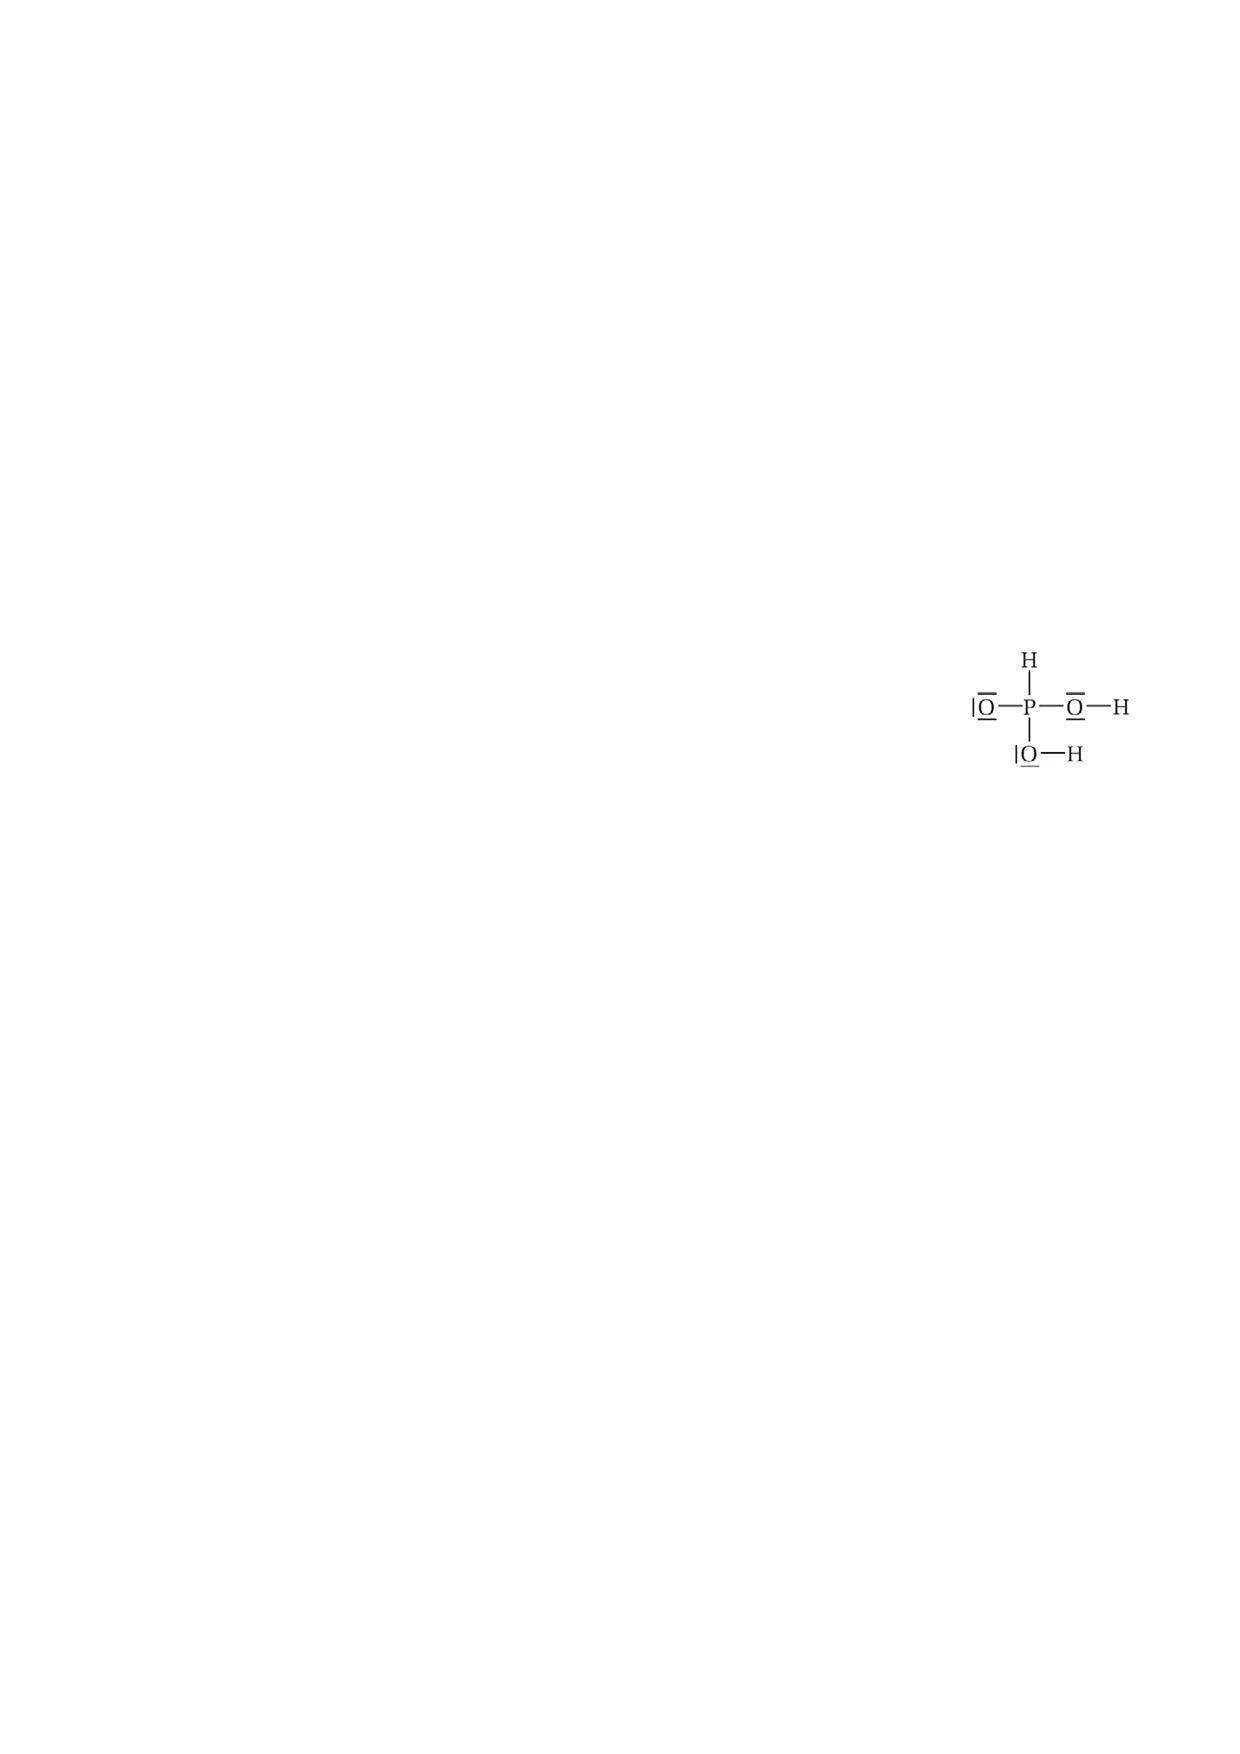
\includegraphics{_images/2.pdf}
		
		}
		
	\end{karte}
%%%%%%%%%%%%%%%%%%%%%%%%%%%%%%%%%%%%%

%%%%%%%%%%%%%%%%%%%%%%%%%%%%%%%%%%%%%
	\begin{karte}{
		
		Berechnen Sie die Konzentration des Fluoridions und den pH-Wert einer L�sung mit 0.20 Mol/L \ce{HF} und 0.10 Mol/L \ce{HCl}. $(K_{S\, HF}=6,8\cdot10^{-4})$
		
		}
		
	\end{karte}
%%%%%%%%%%%%%%%%%%%%%%%%%%%%%%%%%%%%%

%%%%%%%%%%%%%%%%%%%%%%%%%%%%%%%%%%%%%
	\begin{karte}{
		
		Welchen pH-Wert hat eine L�sung aus 0.30 Mol Essigs�ure und 0.30 Mol Natriumacetat, zu denen soviel Wasser gegeben wird, dass 1.0 L L�sung entsteht? $(K_{S\, Essigs\ddot{a}ure}=1,8\cdot10^{-5})$
		
		}
		
	\end{karte}
%%%%%%%%%%%%%%%%%%%%%%%%%%%%%%%%%%%%%

%%%%%%%%%%%%%%%%%%%%%%%%%%%%%%%%%%%%%
	\begin{karte}{
		
		Welchen pH-Wert hat ein Puffer mit 0.12 Mol/L Benzoes�ure und 0.20 Mol/L Natriumbenzoat? $(K_{S\, Benzoes\ddot{a}ure}=6,3\cdot10^{-5})$
		
		}
		
	\end{karte}
%%%%%%%%%%%%%%%%%%%%%%%%%%%%%%%%%%%%%

%%%%%%%%%%%%%%%%%%%%%%%%%%%%%%%%%%%%%
	\begin{karte}{
		
		Berechnen sie den pH-Wert. Der sich einstellt, wenn 45 mL einer 0.100 Mol/L \ce{NaOH}-L�sung zu einer 25 mL einer 0.100 Mol/L Essigs�urel�sung gegeben werden. $(K_{S\, Essigs\ddot{a}ure}=1,8\cdot10^{-5})$
		
		}
		
	\end{karte}
%%%%%%%%%%%%%%%%%%%%%%%%%%%%%%%%%%%%%

%%%%%%%%%%%%%%%%%%%%%%%%%%%%%%%%%%%%%
	\begin{karte}{
		
		Der Wert von $K_{L}$ von \ce{CaF_{2}} ist bei 25�C gleich $3.9\cdot10^{-11}Mol^{3}/L^{3}$. Berechnen Sie die L�slichkeit von \ce{CaF2} in Gramm/Liter.
		
		}
		
	\end{karte}
%%%%%%%%%%%%%%%%%%%%%%%%%%%%%%%%%%%%%

%%%%%%%%%%%%%%%%%%%%%%%%%%%%%%%%%%%%%
	\begin{karte}{
		
		Bildet sich beim Mischen von $0.1L$ $8,0\cdot10^{-3}Mol/L$ \ce{Pb(NO3)2} und $0.4L$ $5,0\cdot10^{-3}$ $Mol/L$ \ce{Na2SO4} ein Niederschlag?
		$(K_{L_{8\ce{PbSO4}}}=6,3\cdot10^{-7}Mol^{2}/L^{2})$ 
		
		}
		
	\end{karte}
%%%%%%%%%%%%%%%%%%%%%%%%%%%%%%%%%%%%%

